\documentclass{article}

\usepackage{setspace} \doublespacing % doublespacing this is required for submission dont change this
\usepackage{floatrow}
\usepackage{graphicx} % Required for inserting images
\usepackage[a4paper, total={6in, 8in}]{geometry}
\usepackage{parskip} % Required to stop indenting new paragraphs
\usepackage{amssymb}
\usepackage{amsmath}
\usepackage{algpseudocode}
\usepackage{algorithm}
\usepackage{pgfplotstable}
\usepackage[hidelinks]{hyperref}
\usepackage{arydshln} % dashed lines in tables
\usepackage[numbers]{natbib} % number references and natbib for more styles
\bibliographystyle{unsrtnat} % sets bibliography to vancouver style

\title{Reverse Mode Algorithmic Differentiation}
\author{Callum Firth, Maximilian Fricker, Alexander Le Marchant, Samuel Murdoch} % alphabetical
\date{June 2023}

\begin{document}

\maketitle

\tableofcontents

\section{Introduction}

Complex computer simulations and models underpin our modern society: being at the heart of a vast number of endeavours such as weather forecasting, modeling of the spread of disease, and machine learning. These models often rely on the computation of a large number of derivatives, in order to assess how changing certain parameters affects the outputs in order to optimise the system. Hence being able to differentiate these programs with a method that is both fast and efficient but also accurate is very important. The method that satisfies these requirements, which we explore in this report, is algorithmic differentiation.

Neural networks consist of many nodes connected by a series of weights that can be adjusted in order to change the output of the model. The algorithm that is most commonly used to find the optimal weights is gradient descent. The goal of gradient descent is to find a local minimum of a cost function that measures the distance between the data predicted by the model and the observed results. It does this by computing the derivative of the cost function with respect to model parameters and then adjusting those parameters such that the derivative reduces in magnitude to get closer to the optimal model. As neural networks are often controlled by thousands or millions of parameters and the number of input parameters is often several magnitudes larger than the number of output variables, it is imperative that a fast and accurate method of differentiation is used, and one which cost does not depend on the number of input variables.

During the computation of computer models and simulations, it is often necessary to solve non-linear systems of equations as the vast majority of real-world systems are not linear. However, in general, it is very difficult to directly solve these systems and so they have to be solved numerically. One such method is Newton's method which relies on calculating derivatives. Say the system is defined by

\begin{equation} \label{Fxy}
        F: \mathbb{R}^n \rightarrow \mathbb{R}^m \qquad F(x_1, \cdots, x_n) = (y_1, \cdots, y_m)
\end{equation}
then given $x_0 \in \mathbb{R}^n$ the iterates are calculated by
\begin{equation}
x_{n+1} = x_n - [F'(x_n)]^{-1}F(x_n) \quad n \in \mathbb{N}
\end{equation}
where $F'(x_n)$ is the Jacobian of $F$ at $x_n$ defined by
\begin{equation} \label{jacobian}
    F'(x) = \begin{bmatrix}
        \frac{\partial y_1}{\partial x_1} & \cdots & \frac{\partial y_1}{\partial x_n} \\
        \vdots & \ddots & \vdots \\
        \frac{\partial y_m}{\partial x_1} & \cdots & \frac{\partial y_m}{\partial x_n}
    \end{bmatrix} \in \mathbb{R}^{m \times n}
\end{equation}

Hence finding the derivative of a function is essential for us to be able to solve our system. So again we need to find a way of computing the derivative of a function at a low cost due to the fact that a high number of iterates will need to be calculated.

From the examples above and those stated in \cite{appad} we see the importance of the implementation of quick derivative computation on computers.

\section{Basics of Computing Derivatives}

There are three common ways to differentiate functions on a computer: numerically, symbolically, and algorithmically. The latter which we will be discussing in depth in this paper. Notably, we will be focusing on reverse mode algorithmic differentiation (AD).

The most common example of numerical differentiation is the finite differences method. For \\ $F: \mathbb{R}^n \longrightarrow \mathbb{R}^m$ in \eqref{Fxy}, a partial derivative can be approximated using a truncated Taylor series around $x \in \mathbb{R}^n$. From \cite{chem}
\begin{equation}
    \frac{\partial F_i (x)}{\partial x_j} \approx \frac{F_i(x+he_j) - F_i(x)}{h}
\end{equation}
This calculation for the derivative is approximate due to the error in the truncated Taylor series. The cost of calculating the Jacobian of $F$ given by \eqref{jacobian} is $\mathcal{O}(n)\cdot \mathrm{Cost}(F)$ where $\mathrm{Cost}(F)$ is the cost of evaluating $F$. Thus, finite differences are unsuited for systems with a large number of input variables. In contrast to symbolic and algorithmic differentiation, numerical differentiation results in an approximation for the derivative.

Symbolic differentiation involves taking an algebraic expression and computing its derivative with respect to a specified variable through repeated application of chain rule, providing the derivative at any $x \in \mathbb{R}^n$. It can be useful as, once the formula for the derivative is computed, finding the value of the derivative at a point is as simple as substituting it into the formula for the derivative.  Furthermore, symbolic differentiation provides an explicit formula for the derivative which is beneficial from a mathematical point of view. However, it has the drawback that it can only be applied when the function to be differentiated exists in a closed form. For calculating the gradient of $F_i$ in \eqref{Fxy}, symbolic differentiation has a computational cost of $n$ times the cost of evaluating $F_i$ \cite{chem}, where $F_i$ is the respective output of $F$. Hence, the computational cost for calculating the Jacobian of a set of equations, defined by $F$, would be prohibitively expensive at $\mathcal{O}(n m)\cdot \mathrm{Cost}(F)$.

There are two forms of AD: forward mode and reverse mode. Similar to symbolic differentiation, the chain rule is fundamental to AD. However, AD only returns the partial derivative at a specified $x \in \mathbb{R}^n$. Calculating the Jacobian in \eqref{jacobian} with forward mode algorithmic differentiation, this has computational cost $\mathcal{O}(n)\cdot \mathrm{Cost}(F)$. In contrast, the computational cost of $[F'(x)]^\text{T}$ with reverse mode algorithmic differentiation is $\mathcal{O}(m)\cdot \mathrm{Cost}(F)$\cite{falisse}. Hence, reverse mode is suited for functions $F$ where $n >> m$, as the cost of reverse mode does not depend on the number of input variables, but on the output variables. We will see below that the reverse mode has an even better complexity error for calculating gradients compared to the alternatives. One drawback of reverse mode algorithmic differentiation over forward mode is that it requires higher memory usage, due to the necessity to store intermediary values \cite{dhamarticle}. However, storing these values beforehand, it provides considerably quicker computation.

\section{Directed Acyclic Graphs to Represent Expressions}

For a function $F: \mathbb{R}^3 \rightarrow \mathbb{R}^2$ defined by
\begin{equation} \label{example1}
    F \begin{pmatrix}
        x \\ y \\ z
    \end{pmatrix} = \begin{pmatrix}
        \sin (x^2 y) + e^{x^2} \\ e^{x^2} \log z
    \end{pmatrix}
\end{equation}
its representation as a Directed Acyclic Graph, DAG, and an expression tree can be seen in Figure \ref{fig:DAGgraph2}.

\begin{figure}[h]
    \centering
    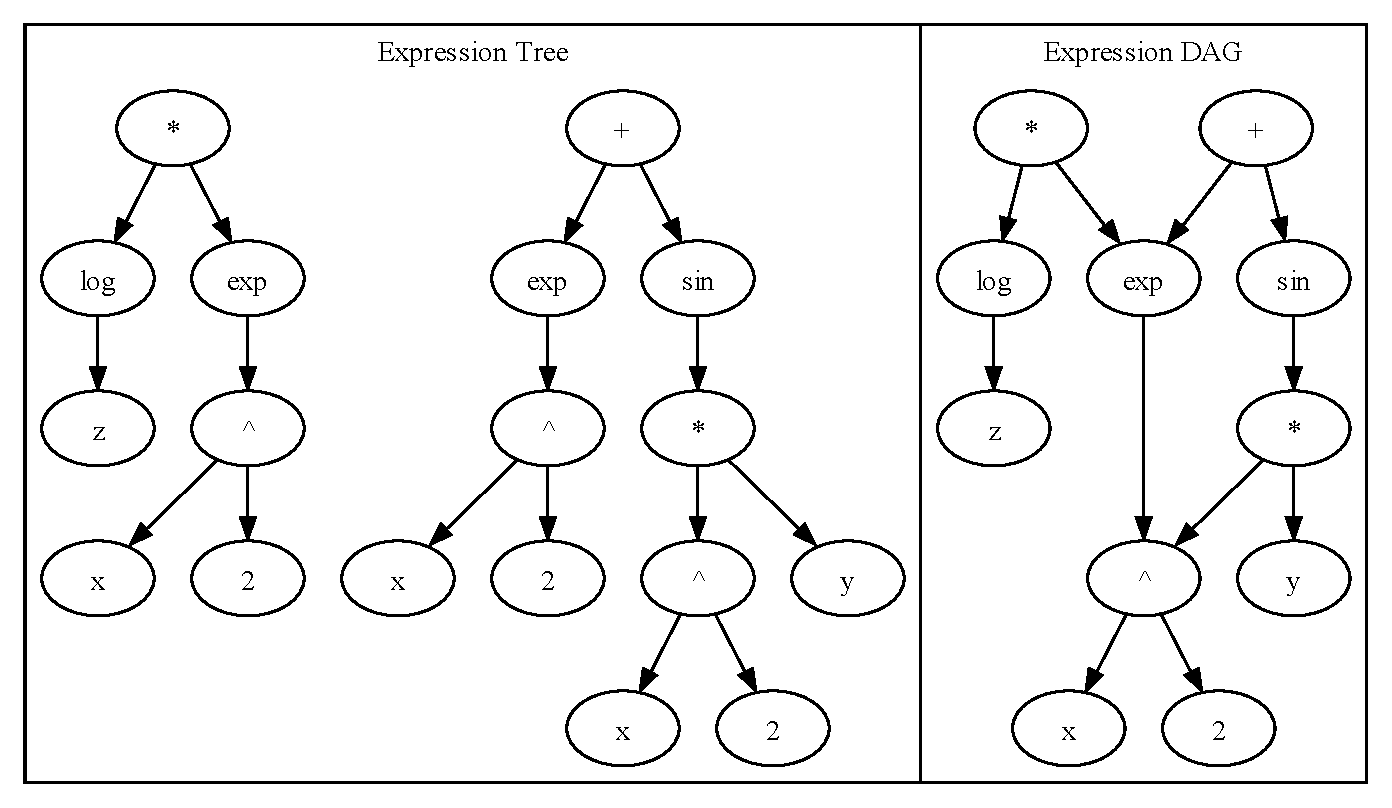
\includegraphics[width=12cm]{images/Graph_Cluster_1.pdf}
    \caption{A DAG and expression tree representation of \eqref{example1}}
    \label{fig:DAGgraph2}
\end{figure}

As in \cite{PoPBook}, we can represent an arithmetic expression as an expression tree. Here we represent each operator, symbol and number in a given expression as nodes in a graph, we denote these as elements. The operands of each element are the children of the node. We will represent links out of a node indicating the children of the node. We can also write an expression as a DAG, which allows us to represent operands as having more than one parent in order to avoid recursion. An example of the difference between the two can be seen in Figure \ref{fig:DAGgraph2}. We from now on will use DAGs to represent expressions as this is essential in lowering runtime and allowing fast computation of complicated expressions as now calculations for shared operands only have to happen once. We will presume that the ordering of each child is important. Representing expressions as DAGs will become important later on when we look at how we can traverse these to evaluate and calculate the derivative of expressions

\section{Fundamentals of Algorithmic Differentiation}

Using notation from \cite{evald}, let $F: \mathbb{R}^n \rightarrow \mathbb{R}^m$ and $F(x) = y$ from \eqref{Fxy}. Assume $F$ is the composition of a sequence and composition of continuously differentiable elemental functions $(\varphi_i)_{i=1,\ldots, l}$, the derivatives of which can be easily calculated. In our case, we will use the elemental functions provided in Table \ref{tab:elemental}.

\begin{table}[h]
    \centering
    \begin{tabular}{|lll|}
        \hline
        Elementary Function $\varphi$ & $\partial \varphi / \partial {v}_1$ & $\partial \partial \varphi / \partial {v}_2$ \\
        \hline
        $v_1+v_2$ & $1$ & $1$ \\
        $v_1-v_2$ & $1$ & $-1$ \\
        $v_1 \times v_2$ & $v_2$ & $v_1$ \\
        $v_1 / v_2$ & $1/v_2$ & $-v_1/v_2^2$ \\
        ${v_1}^{v_2}$ & $v_2{v_1}^{(v_2-1)}$ & ${v_1}^{v_2}\log(v_1)$ \\
        \hdashline
        $\sin(v_1)$ & $\cos(v_1)$ & \\
        $\cos(v_1)$ & $-\sin(v_1)$ & \\
        $\exp(v_1)$ & $\exp(v_1)$ & \\
        $\log(v_1)$ & $1/v_1$ & \\
        \hline
    \end{tabular}
    \caption{Partial Derivatives of Elemental Functions $\varphi$}
    \label{tab:elemental}
\end{table}

The quantities calculated at for our elementary functions are labelled such that
\begin{equation}
    [ \underbrace{v_{1-n}, \ldots, v_0}_{x} , v_1, \ldots, v_{l-m}, \underbrace{v_{l-m+1}, \ldots, v_l}_{y}]
\end{equation}
Using $j \prec i$ to show $v_i$ depends directly on $v_j$, where it is assumed $j \prec i \Longrightarrow j < i$, then it can be written
\begin{equation}
    v_i = \varphi_i (v_j)_{j \prec i} \text{ for } \varphi_i : \mathbb{R}^{n_i} \longrightarrow \mathbb{R}
\end{equation}
We can see our values $v_1, \ldots, v_{l-m}$ can be considered to be our intermediary values.
Here $n_i$ depends on $\varphi_i$. $n_i=1$ or $n_i=2$ for our elementary functions in Table \ref{tab:elemental}, however later we consider examples where this may not be the case.

\subsection{Forward Mode}

We will use the interpretation of forward mode AD given in \cite{dhamarticle}. Assume $x$ is equal to the value a time-dependent $x(t)$ takes at $t=0$. Then define the tangent
\begin{equation}
    \dot{x} = \frac{\partial x}{\partial t} \Big|_{t=0}
\end{equation}
As $y = F(x)$ we calculate the tangent $\dot{y}$ as
\begin{equation}
    \Dot{y} = \frac{\partial}{\partial t} F(x (t)) \Big|_{t=0} 
    = F'(x (t)) \cdot \frac{\partial x}{\partial t} \Big|_{t=0}
    = F'(x) \cdot \Dot{x}
    \equiv \Dot{F}(x, \Dot{x})
\end{equation}
Using the additional notation $u_i = (v_j)_{j \prec i}$ and $\Dot{u}_i = (\Dot{v}_j)_{j \prec i}$, the idea can be applied to an elemental function $\varphi_i : \mathbb{R}^{n_i} \longrightarrow \mathbb{R}$, $v_i = \varphi_i (u_i)$ to get the result
\begin{equation} 
    \Dot{v_i} = \nabla \varphi_i (u_i) \cdot \Dot{u}_i
    \equiv \Dot{\varphi}_i(u_i, \Dot{u}_i)
\end{equation} 
This can be rewritten in summation form as
\begin{equation} \label{tangentequ}
    \Dot{v_i} = \sum_{j \prec i} \left\{ \Dot{v}_j \cdot \frac{\partial}{\partial v_j} \varphi_i (u_i) \right\} 
\end{equation}
This can be summarised as the general evaluation procedure from \cite{evald} and given in Table \ref{tab:gep}.
This shows the assignment for all the input, intermediate and output variables

\begin{table}[h]
    \centering
    \begin{tabular}{|lcll|}
        \hline
        $v_{i-n}$ & $\equiv$ & $x_i$ & $i = 1, \ldots, n$ \\
        \hline
        $v_{i}$ & $\equiv$ & $v_i = \varphi_i (u_i)$ & $i = 1, \ldots, l$ \\
        \hline
        $v_{l-m+i}$ & $\equiv$ & $y_i$ & $i = 1, \ldots, m$ \\
        \hline
    \end{tabular}
    \caption{General Evaluation Procedure}
    \label{tab:gep}
\end{table}

Because in forward mode we can calculate both the values and the tangents of our elementary function at the same time we can get a more concise procedure for computing the tangents of our function. This is given in Table \ref{tab:gtp}.

\begin{table}[h]
    \centering
    \begin{tabular}{|lcll|}
        \hline
        $[v_{i-n}, \Dot{v}_{i-n}]$ & $=$ & $[x_{i}, \Dot{x}_{i}]$ & $i = 1, \ldots, n$ \\
        \hline
        $[v_{i}, \Dot{v}_{i}]$ & $=$ & $[\varphi_i (u_i), \Dot{\varphi}_i(u_i, \Dot{u}_i)]$ & $i = 1, \ldots, l$ \\
        \hline
        $[v_{l-m+i}, \Dot{v}_{l-m+i}]$ & $=$ & $[y_{i}, \Dot{y}_{i}]$ & $i = 1, \ldots, m$ \\
        \hline
    \end{tabular}
    \caption{General Tangent Procedure}
    \label{tab:gtp}
\end{table}

\subsection{Reverse Mode}

As in \cite{dhamarticle}, consider for the image of $F$ the hyperplane $\{ y \in \mathbb{R}^m | \Bar{y}^\text{T} y = c\}$ for a given vector $\Bar{y} \in \mathbb{R}^m$ and a given value $c \in \mathbb{R}$. The inverse image of this hyperplane is given by the set $\{ x \in \mathbb{R}^n | \Bar{y}^\text{T} F(x) = c\}$. We can apply the implicit function theorem to this set to calculate the normal to this hyperplane at $x$ as
\begin{equation}
    \Bar{x}^\text{T} = \Bar{y}^\text{T} \cdot F'(x) \equiv \Bar{F}(x, \Bar{y})
\end{equation}
This calculation is provided $\Bar{x}^\text{T}$ does not vanish.

Using the additional notation $\Bar{u}_i = (\Bar{v}_j)_{j \prec i}$, we calculate the adjoint function for each elemental function $\varphi_i : \mathbb{R}^{n_i} \longrightarrow \mathbb{R}$ as
\begin{equation}
    \Bar{u}_i += \Bar{v}_i \cdot \nabla \varphi_i (u_i)
\end{equation}
In notation similar to \eqref{tangentequ}
\begin{equation}
    \Bar{v}_i = \sum_{j \succ i} \left\{ \Bar{v}_j \cdot \frac{\partial}{\partial v_i} \varphi_j(u_j) \right\}
\end{equation}
In reverse mode, we first evaluate our function starting with our inputs first, calculating the value of each elemental function until the outputs. Then, we work backwards, calculating the adjoint of each elemental function starting with the outputs first. Using all the notation above, this produces the adjoint procedure for computing the first derivative from \cite{dhamarticle}, given in Table \ref{tab:ap}. 
\begin{table}[h]
    \centering
    \begin{tabular}{|llll|}
        \hline
        $v_{i}$ & $=$ & $0$ & $i = 1, \ldots, l$ \\
        \hline
        $[v_{i-1}, \Bar{v}_{i-1}]$ & $=$ & $[x_{i}, \Bar{x}_{i}]$ & $i = 1, \ldots, n$ \\
        \hline
        push$(v_i)$ & & & \\
        $v_{i}$ & $=$ & $v_i = \varphi_i (u_i)$ & $i = 1, \ldots, l$ \\
        \hline
        $v_{l-i}$ & $=$ & $y_{m-1}$ & $i = 1, \ldots, m-1$ \\
        $\Bar{v}_{l-i}$ & $=$ & $\bar{y}_{m-1}$ & $i = 1, \ldots, m-1$ \\
        \hline
        $v_i \leftarrow$ pop$()$ & & & \\
        $\Bar{u}_i$ & $+=$ & $\Bar{v}_i \nabla \varphi_i (u_i)$ & $i = l, \ldots, 1$ \\
        $v_i$ & $=$ & $0$ & \\
        \hline
        $\Bar{v}_{i-n}$ & $=$ & $\Bar{x}_i$ & $i = 1, \ldots, n$ \\
        \hline
    \end{tabular}
    \caption{General Adjoint Procedure}
    \label{tab:ap}
\end{table}

\section{Complexity Results for Algorithmic Differentiation}

Below we will use notation and results from \cite{dhamarticle} for the number of operations and the memory usage required to compute a function. The number of operations is denoted $\text{OPS}(\cdot)$. The amount of random access memory and the amount of sequentially accessed memory are denoted $\text{RMEM}(\cdot)$ and $\text{SMEM}(\cdot)$ respectively. 

\subsection{Forward Mode}

Given $x, \Dot{x} \in \mathbb{R}^n$ we attain an upper bounded for calculating the number of operations required to compute $F'(x) \Dot{x}$, a column of the jacobian $F'(x)$, given in \eqref{ops1}. Given an upper bound on the time taken to compute one operation, calculating the bound for the time taken to compute $F'(x)\Dot{x}$ is simple.
\begin{equation} \label{ops1}
    \text{OPS}(F'(x) \cdot \Dot{x}) \leq 3 \cdot \text{OPS}(F(x))
\end{equation}
Further, we get an exact value for the memory requirement in \eqref{rmem1}.
\begin{equation} \label{rmem1}
    \text{RMEM}(F'(x) \cdot \Dot{x}) = 2 \cdot \text{RMEM}(F(x))
\end{equation}

\subsection{Reverse Mode}

Given $x \in \mathbb{R}^n$ and $\Bar{y} \in \mathbb{R}^m$ we attain an upper bound for calculating the number of operations required to compute $\Bar{y}^\text{T} F'(x)$, a row of the jacobian $F'(x)$, given in \eqref{ops2}. Similarly to before, an upper bound for the time taken to compute $\Bar{y}^\text{T} F'(x)$ can be calculated provided we know the time taken to compute one operation.
\begin{equation} \label{ops2}
    \text{OPS}(\Bar{y}^\text{T} \cdot F'(x)) \leq 4 \cdot \text{OPS}(F(x))
\end{equation}
The memory usage is given in \eqref{rmem2}. Here we see the random access memory usage is the same as forward mode but the use of sequentially accessed memory creates an overall memory usage increase.
\begin{equation} \label{rmem2}
    \begin{gathered}
        \text{RMEM}(\Bar{y}^\text{T} \cdot F'(x)) = 2 \cdot \text{RMEM}(F(x)) \\ 
        \text{SMEM}(\Bar{y}^\text{T} \cdot F'(x)) \approx \text{OPS}(F(x))
    \end{gathered}
\end{equation}

\section{Applying Algorithmic Differentiation on Directed Acyclic Graphs}

If we consider an expression represented by a DAG, then it is very easy to apply the concept of forward and reverse mode AD. Here we can represent each element/node denoted $v_i$ as our elementary function $v_i = \varphi_i (v_j)_{j \prec i}$ where now we can view $j \prec i$ to mean that $v_j$ is an operand of $v_i$. Then to apply forward mode we can compute our tangents in \eqref{tangentequ} by traversing this graph with post-order traversal, visiting child nodes before the parent, calculating both the values, $v_i$, and the tangent values, $\Dot{v_i}$ as we go along. So for one pass/traversal, we can calculate the derivatives of all the output variables w.r.t. one input variable. This is because we start with our input variables first, so we can only seed one of our input variables per traversal of the graph.

Alternatively, we can do reverse mode by first traversing postorder traversal on the graph, computing all the values, $v_i$. Then we can preorder traverse, visiting the parents before the child nodes, on the graph to compute the adjoint of each variable as we go along. So for one pass, we can calculate the adjoint of one output variable with respect to every input variable. This is because we start with our output variables first we can only seed one output variable per traversal of the graph.

This gives us an idea of why forward mode has a computational cost proportional to $n$, as we require to have $n$ forward passes to compute the derivative. Similarly, we can see why reverse mode has a computational cost proportional to $m$, as we require to have $m$ reverse passes in order to calculate the derivative. Here we refer to a forward pass as the postorder traversal on an expression and a reverse pass as the preorder traversal on an expression.

For the examples below we will be calculating the partial derivatives at $x=2, y=2$ for \eqref{ADexample}. We will show the computation of both forward and reverse mode AD. We can also represent the equation as a DAG given by Figure \ref{fig:DAGgraph}

\begin{equation}
    \label{ADexample}
    F(x,y) = \sin(x^2y) + e^{x^2}
\end{equation}

\begin{figure}[h!]
    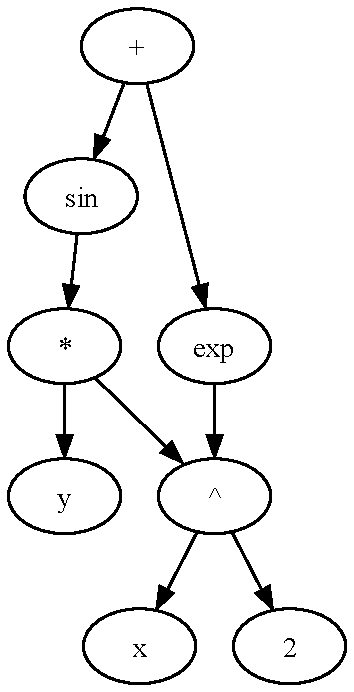
\includegraphics[width=4cm]{images/Graph_Example2.pdf}
    \caption{DAG of \eqref{ADexample}}
    \label{fig:DAGgraph}
\end{figure}

\subsection{Example of Forward Mode}

First, we will label our nodes and respective tangents for our expression as seen in Table \ref{tab:fexample1}. To calculate $\partial F / \partial x$ we need to seed our input variables, we first seed $x$ so we set $\dot{x}=1$ and $\dot{y}=0$ then simultaneously compute the node values and tangents listed in Table \ref{tab:fexample1} by traversing the graph with postorder traversal. To calculate $\partial F / \partial y$ we do the same process but we seed $y$ first, so we start with $\dot{x}=0$ and $\dot{y}=1$. Note we do not need to recalculate the values of $v_i \ i \in \{1-n, \ldots, l \}$ as they have been stored when calculating $\partial F / \partial x$. In Table \ref{tab:fexample1FP} we label these Pass 1 and Pass 2 respectively.

\begin{table}[h!]
    \centering
    \begin{tabular}{|lcl|lclll|}
        \hline
        Elementary Function & & & Tangent & & & & \\
        \hline
        $v_{-1}$ & $\equiv$ & $x$ & $\dot{v}_{-1}$ & $=$ & $\dot{x}$ & $=$ & $\dot{x}$\\
        $v_{0}$ & $\equiv$ & $y$ & $\dot{v}_{0}$ & $=$ & $\dot{y}$ & $=$ & $\dot{y}$\\
        \hline
        $v_{1}$ & $=$ & $2$ & $\dot{v}_{1}$ & $=$ & $0$ & $=$ & $0$\\
        $v_{2}$ & $=$ & ${v_{-1}}^{v_{1}}$ & $\dot{v}_{2}$ & $=$ & $\dot{v_1}\frac{\partial{v_2}}{\partial{v_1}} + \dot{v}_{-1}\frac{\partial{v_2}}{\partial{v_{-1}}}$ & $=$ & $2v_{-1}\dot{v}_{-1}$\\
        $v_{3}$ & $=$ & ${v_{0}}*{v_{2}}$ & $\dot{v}_{3}$ & $=$ & $\dot{v_0}\frac{\partial{v_3}}{\partial{v_0}} + \dot{v}_{2}\frac{\partial{v_3}}{\partial{v_{2}}}$ & $=$ & $v_2\dot{v}_{0}+v_{0}\dot{v}_2$\\
        $v_{4}$ & $=$ & $\sin(v_3)$ & $\dot{v}_{4}$ & $=$ & $\dot{v}_3\frac{\partial{v_4}}{\partial{v_3}}$ & $=$ & $\dot{v}_3 \cos (v_3)$\\
        $v_{5}$ & $=$ & $e^{v_2}$ & $\dot{v}_{5}$ & $=$ & $\dot{v_2}\frac{\partial{v_5}}{\partial{v_2}}$ & $=$ & $\dot{v}_2 e^{v_2}$\\
        \hline
        $v_{6}$ & $=$ & $v_4 + v_5$ & $\dot{v}_{6}$ & $=$ & $\dot{v}_4 \frac{\partial v_6}{\partial v_4} + \dot{v}_5 \frac{\partial v_6}{\partial v_5}$ & $=$ & $\dot{v}_4 + \dot{v}_5$\\
        \hline
    \end{tabular}
    \caption{Table of Node Values and Tangents in Figure \ref{fig:DAGgraph} of \eqref{ADexample}}
    \label{tab:fexample1}
\end{table}

\begin{table}[h]
    \centering
    \begin{tabular}{|lclcll|}
        \hline
        Elementary function & & Value, Tangent & & Pass 1 & Pass 2 \\
        \hline
        $[v_{-1}, \dot{v}_{-1}]$ & $=$ & $[x, \Dot{x}]$ & $=$ & $[2,1]$ & $[2,0]$ \\
        $[v_{0}, \dot{v}_0]$ & $=$ & $[y, \dot{y}]$ & $=$ & $[2,0]$ & $[2,1]$ \\
        \hline
        $[v_{1}, \dot{v}_1]$ & $=$ & $[2, 0]$ & $=$ & $[2,0]$  & $[\cdot,0]$\\
        $[v_{2}, \dot{v}_2]$ & $=$ & $[{v_{-1}}^{v_1}, 2v_{-1}\dot{v}_{-1}]$ & $=$ & $[4,4]$ & $[\cdot,0]$\\
        $[v_{3}, \dot{v}_3]$ & $=$ & $[v_0 * v_2, v_2\dot{v}_{0}+v_{0}\dot{v}_2]$ & $=$ & $[8, 8]$ & $[\cdot, 4]$\\
        $[v_{4}, \dot{v}_4]$ & $=$ & $[\cdot, \dot{v}_3 \cos(v_3)]$ & $=$ & $[\sin(8),8\cos(8)]$ & $[\cdot,4\cos(8)]$\\
        $[v_{5}, \dot{v}_5]$ & $=$ & $[e^{v_2}, \dot{v}_2 e^{v_2}]$ & $=$ & $[e^4,4e^4]$ & $[\cdot,0]$\\ 
        \hline
        $[v_{6}, \dot{v}_6]$ & $=$ & $[v_4 + v_5, \dot{v}_4 + \dot{v}_5]$ & $=$ & $[e^4 + \sin(8),4e^4 + 8\cos(8)]$ & $[\cdot,4\cos(8)]$\\
        \hline
    \end{tabular}
    \caption{Calculation of values and tangents for forward mode AD for \eqref{ADexample}}
    \label{tab:fexample1FP}
\end{table}

Hence from Table \ref{tab:fexample1FP} we get expressions for the partial derivatives given in \eqref{fmexample1results}.

\begin{equation} \label{fmexample1results}
    \begin{gathered}
        \frac{\partial F}{\partial x} = \Dot{v}_{6} = 8\cos(8) + 4e^4 \approx 217.228599862 \\
        \frac{\partial F}{\partial y} = \Dot{v}_{6} =  4\cos(8) \approx -0.58200013523
    \end{gathered}
\end{equation}

\subsection{Example of Reverse Mode}

Now let's look at how we would use reverse mode AD to compute the adjoints. Here we label the nodes according to Table \ref{tab:rmexample1}. We first traverse the graph in postorder traversal, computing the values of each node as we go along. The results after this first forward pass are seen in Table \ref{tab:rmexample1FP}. After the forward pass we can now we calculate the adjoints of our nodes, we first do this by seeding the output variable, so we set $\Bar{v}_6 = 1$ and then traverse the graph with preorder traversal, calculating the adjoints of each node as we do along, using the intermediary values we calculated on the first pass. The results after this reverse pass are seen in Table \ref{tab:rmexample1RP}. Note that in reverse mode we only needed to do one reverse sweep to get adjoints of all the inputs, compared to forward mode of which we had to sweep separately for each input.

\begin{table}[h!]
    \centering
    \begin{tabular}{|lcl|lclll|}
        \hline
        Elementary function & & & Adjoint & & & &\\
        \hline
        $v_{-1}$ & $\equiv$ & $x$ & $\Bar{v}_{-1}$ & $=$ & $\Bar{v_2}\frac{\partial{v_2}}{\partial{v_{-1}}}$ & $=$ & $\Bar{v_2}v_1 {v_{-1}}^{(v_{1}-1)}$\\
        $v_{0}$ & $\equiv$ & $y$ & $\Bar{v}_{0}$ & $=$ & $\Bar{v_3}\frac{\partial{v_3}}{\partial{v_0}}$ & $=$ & $\Bar{v_3}v_2$\\
        \hline
        $v_{1}$ & $=$ & $2$ & $\Bar{v}_{1}$ & $=$ & $\Bar{v_2}\frac{\partial{v_2}}{\partial{v_1}}$ & $=$ & $\Bar{v}_{2}{v_{-1}}^{v_{1}}\log(v_{-1})$\\
        $v_{2}$ & $=$ & ${v_{-1}}^{v_{1}}$ & $\Bar{v}_{2}$ & $=$ & $\Bar{v_3}\frac{\partial{v_3}}{\partial{v_2}} + \Bar{v_5}\frac{\partial{v_5}}{\partial{v_2}}$ & $=$ & $\Bar{v}_{3}v_0 + \Bar{v_5}e^{v_2}$\\
        $v_{3}$ & $=$ & ${v_{0}}*{v_{2}}$ & $\Bar{v}_{3}$ & $=$ & $\Bar{v_4}\frac{\partial{v_4}}{\partial{v_3}}$ & $=$ & $\Bar{v_4}\cos(v_2)$\\
        $v_{4}$ & $=$ & $\sin(v_3)$ & $\Bar{v}_{4}$ & $=$ & $\Bar{v_6}\frac{\partial{v_6}}{\partial{v_4}}$ & $=$ & $\Bar{v_6}$\\
        $v_{5}$ & $=$ & $e^{v_2}$ & $\Bar{v}_{5}$ & $=$ & $\Bar{v_6}\frac{\partial{v_6}}{\partial{v_5}}$ & $=$ & $\Bar{v_6}$\\
        \hline
        $v_{6}$ & $=$ & $v_5 + v_4$ & $\Bar{v}_{6}$ & $=$ & $\frac{\partial{v_6}}{\partial{v_6}}$ & $=$ & $1$\\
        \hline
    \end{tabular}
    \caption{Table of Node Values and Adjoints in Figure \ref{fig:DAGgraph} of \eqref{ADexample}}
    \label{tab:rmexample1}
\end{table}

\begin{table}[h!]
    \centering
    \begin{tabular}{|lclllcl|}
        \hline
        Elementary Function & & & & Value & &\\
        \hline
        $v_{-1}$ & $=$ & $x$ & $\equiv$ & 2 & $=$ & 2\\
        $v_{0}$ & $\equiv$ & $y$ & $\equiv$ & 2 & $=$ & 2\\
        \hline
        $v_{1}$ & $\equiv$ & $2$ & $=$ & 2 & $=$ & 2\\
        $v_{2}$ & $\equiv$ & ${v_{-1}}^{v_{1}}$ & $=$ & $ 2^2$ & $=$ & $4$\\
        $v_{3}$ & $\equiv$ & $v_0 * v_2$ & $=$ & $ 2 \cdot 4$ & $=$ & $8$\\
        $v_{4}$ & $\equiv$ & $\sin(v_3)$ & $=$ & $\sin(8)$ & $\approx$ & $0.9894$\\
        $v_{5}$ & $\equiv$ & $e^{v_2}$ & $=$ & $ e^4$ & $\approx$ & $54.5982$\\
        \hline
        $v_{6}$ & $\equiv$ & $v_5 + v_4$ & $=$ & $e^4 + \sin(8)$ & $\approx$ & $55.5875$\\
        \hline
    \end{tabular}
    \caption{Values of Figure \ref{fig:DAGgraph} After Forward Pass}
    \label{tab:rmexample1FP}
\end{table}

\begin{table}[h!]
    \centering
    \begin{tabular}{|lclll|}
        \hline
        Adjoint & & & & \\
        \hline
        $\Bar{v}_{6}$ & $=$ & $1$ & $=$ & $1$ \\
        \hline
        $\Bar{v}_{5}$ & $=$ & $\Bar{v_6}$ & $=$ & $1$\\
        $\Bar{v}_{4}$ & $=$ & $\Bar{v_6}$ & $=$ & $1$\\
        $\Bar{v}_{3}$ & $=$ & $\Bar{v_4}\cos(v_3)$ & $=$ & $1 \cdot \cos(8) = \cos(8)$ \\
        $\Bar{v}_{2}$ & $=$ & $\Bar{v}_{3}v_0 + \Bar{v_5}e^{v_2}$ & $=$ & $\cos(8) \cdot 2 + 1 \cdot e^{4} = 2\cos(8)+e^4$ \\
        $\Bar{v}_{1}$ & $=$ & $\Bar{v}_{2}{v_{-1}}^{v_{1}}\log(v_{-1})$ & $=$ & $4(2\cos(8)+e^4)\log(2)$ \\
        \hline
        $\Bar{v}_{0}$ & $=$ & $\Bar{v_3}v_2$ & $=$ & $\cos(8)\cdot4 = 4\cos(8)$ \\
        $\Bar{v}_{-1}$ & $=$ & $\Bar{v_2}v_1 {v_{-1}}^{(v_{1}-1)}$ & $=$ & $(2\cos(8)+e^4) \cdot 2 \cdot 2^{2-1} = 8\cos(8)+4e^4$ \\
        \hline   
    \end{tabular}
    \caption{Adjoints of Figure \ref{fig:DAGgraph} After Reverse Pass}
    \label{tab:rmexample1RP}
\end{table}

From Table \ref{tab:rmexample1RP} we get expressions for the partial derivatives given in \eqref{rmexample1RPresults}. We see these  match the  derivatives calculated in forward mode.

\begin{equation} \label{rmexample1RPresults}
    \begin{gathered}
    \frac{\partial F}{\partial x} = \Bar{v}_{-1} = 8\cos(8) + 4e^4 \approx 217.228599862 \\
    \frac{\partial F}{\partial y} = \Bar{v}_0 =  4\cos(8) \approx -0.58200013523
    \end{gathered}
\end{equation}

\section{Implementation of Scalar Reverse Mode in Python}

To implement reverse mode AD in Python we used the symbolic language defined in \cite{PoPBook} as a template. This allowed us to have a symbolic language that we could use to easily construct our expressions. It does this by operator overloading our elementary operators so we can easily create an expression that we can traverse. Here we add additional elementary functions Sin, Cos, Exp and Log. In order to allow them to work with our current expressions class, we modify our base Expression class to contain the following attributes \cite{github}:
\begin{verbatim}
    class Expression:
        def __init__(self, *operands):
            self.operands = operands
            self.storedvalue = 0
            self.adjoint = 0
\end{verbatim}
This allows us to store the intermediate value of our element as we traverse our DAG in our forward pass to use when calculating the adjoints in our reverse pass. We also modified the \verb|evaluate()| function from \cite{PoPBook} to include evaluation of our new functions Sin, Cos, Exp and Log. From \cite{github} here is the code for the evaluate method when the type of our element is Sin()
\begin{verbatim}
    @evaluate.register(expressions.Sin)
    def _(expr, *o, **kwargs):
        return np.sin(o[0])  # o[0] is storedvalue of operand 0
\end{verbatim}

Then we have to create an algorithm for traversing and evaluating the DAG at each node. Note here we need to traverse the DAG in postorder traversal, where we visit the operands before we visit the element. Note, in the implementation we keep a dictionary of the expressions and the stored values in order to make the traversal non-recursive so we can avoid unnecessary calculation. This can be seen in Algorithm \ref{EvaluatePostvisitor}.

\begin{algorithm}[h!]
\caption{EvaluatePostvisitor function}\label{EvaluatePostvisitor}
\begin{algorithmic}[1]
\Procedure{EvaluatePostvisitor}{$expression,conditions$}
\For{each element in expression}\Comment{Postorder traversal: visiting element after its operands}
\State \verb|value| $\gets$ \verb|evaluate(element, operands, conditions)|
\State \verb|element.storedvalue| $\gets$ \verb|value|
\EndFor
\EndProcedure
\end{algorithmic}
\end{algorithm}

Now that we have done a postorder traversal of our expression, each element contains a correct \verb|element.storedvalue| attribute based on its elementary function and our conditions. Now we need to do a preorder traversal of our graph, evaluating the adjoint at each node. To do this we need to create a new \verb|adjoint_evaluate()| method similar to the previous \verb|evaluate()| method but instead it will calculate the adjoint of each of the operands with respect to the element, the Table \ref{tab:AdjEval} shows the output of \verb|adjoint_evaluate()| based on each element. Presume $w_1$ and $w_2$ are \verb|v_1.storedvalue| and \verb|v_2.storedvalue| respectively for $v_1$ and $v_2$ operands of \verb|element|. Note $\sin()$, $\cos()$, etc only have one operand and thus only one output. Also we denote $v_\mathrm{adj}$ the adjoint of \verb|element|. While it might seem unnecessary to multiply each case by the current adjoint, it is necessary as later we may not have linearity.

\begin{table}[h!]
    \centering
    \begin{tabular}{|lll|}
        \hline
        Type of \verb|element| & Operand 1  & Operand 2 \\
        \hline
        Add() & $v_\mathrm{adj}\cdot $1 & $v_\mathrm{adj}\cdot $1 \\
        Sub() & $v_\mathrm{adj}\cdot $1 & $v_\mathrm{adj}\cdot $-1 \\
        Mul() & $v_\mathrm{adj}\cdot w_2$ & $v_\mathrm{adj}\cdot w_1$ \\
        Div() & $v_\mathrm{adj}\cdot 1/w_2$ & $v_\mathrm{adj}\cdot (-w_1/w_2^2)$ \\
        Pow() & $v_\mathrm{adj}\cdot w_2{w_1}^{(w_2-1)}$ & $v_\mathrm{adj}\cdot {w_1}^{w_2}\log(w_1)$ \\
        \hdashline
        Sin() & $v_\mathrm{adj}\cdot \cos(w_1)$ &  \\
        Cos() & $v_\mathrm{adj}\cdot (-\sin(w_1))$ &  \\
        Exp() & $v_\mathrm{adj}\cdot \exp(w_1)$ &  \\
        Log() & $v_\mathrm{adj}\cdot 1/w_1$ &  \\
        \hline
    \end{tabular}
    \caption{Output of \verb|adjoint\_evaluate(element)| \cite{github}}
    \label{tab:AdjEval}
\end{table}

Now we can run \verb|adjoint_evaluate()| method at each element when traversing the expression tree in preorder traversal, visiting the element before its operands. In order to compute the adjoint of our expression. This can be seen in Algorithm \ref{AdjointPrevisitor}.

\begin{algorithm}[h]
\caption{AdjointPrevisitor function}\label{AdjointPrevisitor}
\begin{algorithmic}[1]
\Procedure{AdjointPrevisitor}{$expression$, adjoint=1}
\State \verb|expression.adjoint| $\gets$ adjoint
\State \verb|adjoint| $=$ \verb|adjoint_evaluate(expression, operands)|\Comment{adjoint is a list}
\For{each index,operand in enumerate(expressions.operand)}\Comment{Preorder traversal}
\State \verb|operand.adjoint| $+=$ \verb|adjoint[index]|
\State run \verb|AdjointPrevisitor(operand, operand.adjoint)|
\EndFor
\EndProcedure
\end{algorithmic}
\end{algorithm}

Now we have populated all the elements with their respective adjoints and so we can simply return a dictionary of all the symbols and their adjoint values to get the partial derivatives of our original expression. So now we can simply define a new function to calculate the derivative of an expression given some conditions. The general idea of this function is seen in Algorithm \ref{reverseAD}.

\begin{algorithm}[h]
\caption{ReversemodeAD algorithm}\label{reverseAD}
\begin{algorithmic}[1]
\Procedure{ReversemodeAD}{$expression,conditions$}
\State run \verb|EvaluatePostvisitor(expression, conditions)|
\State run \verb|AdjointPrevisitor(expression)|
\State \textbf{return} a dictionary of Symbols and their respective \verb|adjoints|
\EndProcedure
\end{algorithmic}
\end{algorithm}

Now we can test our implementation on the previous example given in \eqref{ADexample} represented by the DAG in Figure \ref{fig:DAGgraph}. We create the code for this like below.

\begin{verbatim}
    x = expressions.Symbol('x')
    y = expressions.Symbol('y')
    x2 = x**2  # Create shared expression
    expression = sin(y * x2) + exp(x2)
    conditions = {x:2, y:2}
    reversemodeAD(expression, conditions)
\end{verbatim}

Running the code above gives us the output below \cite{github}. The values for the derivatives agree with those in \eqref{fmexample1results} and \eqref{rmexample1RPresults}. Hence we know our implementation for the example is correct.
\begin{verbatim}
    > {'x': 217.22859986210804, 'y': -0.5820001352344542}
\end{verbatim}

\section{Taylor Tests}

To further prove we have the correct results and that our implementation of our code is correct, we use the Taylor test. We know from the Taylor series expansion that we have the equation
\begin{equation}
    F(x + \varepsilon) = F(x) + \frac{dF}{dx} \cdot \varepsilon + \mathcal{O}(\varepsilon ^ 2)
\end{equation}
As $\varepsilon \longrightarrow 0$, the term $\mathcal{O}(\varepsilon) \longrightarrow 0$. Meaning we can find $\mathcal{O}(\varepsilon^2)$ by rearranging the equation to get

\begin{equation}
    F(x + \varepsilon) - F(x) - \frac{dF}{dx} \cdot \varepsilon = \mathcal{O}(\varepsilon^2)
\end{equation}

When we compute this we get a value for $\mathcal{O}(\varepsilon^2)$ which as $\varepsilon \longrightarrow 0$, $\mathcal{O}(\varepsilon^2) \longrightarrow 0$ at a rate proportional to $\varepsilon^2$.

\begin{figure}[h!]
    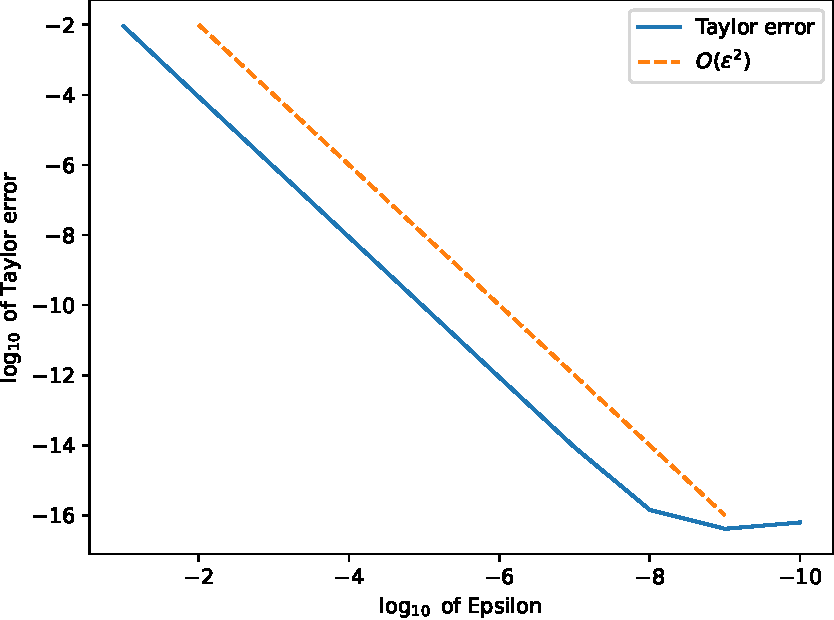
\includegraphics[width=12cm]{images/taylor_error_1.pdf}
    \caption{Plot of Taylor error against epsilon from \cite{github}}
    \label{fig:taylorerror}
\end{figure}

When checking if our result is correct we need to calculate the rate of convergence, since we are finding $\mathcal{O}(\varepsilon^2)$ we expect our convergence to be at the rate of $\varepsilon^2$. To check our rate of convergence we use the formula from \cite{finite}, given in \eqref{taylort}.

\begin{equation} \label{taylort}
   \frac{\log{\frac{\|u_1 - u\|}{\|u_2 - u\|}}}{\log{\frac{|h_1|}{|h_2|}}} = \frac{\log\|u_1 - u\| - \log\|u_2 - u\|}{\log|h_1| - \log|h_2|}
\end{equation}

Where $u_1, u_2$ are our approximations using $F(x + \varepsilon) - F(x)$, $u$ is our calculated derivative using Reverse Mode AD, and $h_1, h_2$ are the corresponding $\varepsilon$ for $u_1, u_2$. This value should give us the power of $\varepsilon$ to which we are converging at. In our case, we got the values provided in Table \ref{tab:taylor-error-values} \cite{github}.

\begin{table}[h]
    \begin{center}
    \pgfplotstabletypeset[
    columns/0/.style={column name={Points Pair}},
    columns/1/.style={column name={Gradients}},
    header=false,
    string type,
    before row=\hline,
    every last row/.style={after row=\hline},
    column type/.add={|}{},
    every last column/.style={column type/.add={}{|}}
    ]{images/rate_of_convergence.txt}%
    \end{center}
    \caption{Gradient of Taylor Error in Figure \ref{fig:taylorerror}}
    \label{tab:taylor-error-values}
\end{table}


As you can see at nearly all points we got values significantly close to 2. So we can conclude convergence at a rate of $\varepsilon^2$.


\section{Extension and Implementation using NumPy Arrays}

Now we consider our expression as being a function of $F: \mathbb{R}^n \longrightarrow \mathbb{R}^m$. We cannot do this with our current implementation. Instead, we represent our expression as a NumPy 1 x m array, where each element of our array consists of the corresponding output. We can now change our algorithms for evaluating the value and adjoint so they work with this change, this involves simply running our reversemode algorithm for each subexpression in our array, and making sure to record the adjoints of each of the symbols at each subexpression. The modified algorithms are seen in Algorithm \ref{reverseADArr} and \ref{EvaluatePostvisitorArr}. Noting that our postvisitor traversal we use is still non-recursive.

\begin{algorithm}[h]
\caption{ReversemodeAD algorithm for arrays}\label{reverseADArr}
\begin{algorithmic}[1]
\Procedure{ReversemodeAD}{$expression,conditions$}
\State run \verb|EvaluatePostvisitor(expression, conditions)|
\For{each subexpression in expression}
\State run \verb|AdjointPrevisitor(subexpression)|
\EndFor
\State \textbf{return} a dictionary of Symbols and their respective \verb|adjoints| for each subexpression
\EndProcedure
\end{algorithmic}
\end{algorithm}

\begin{algorithm}[h!]
\caption{EvaluatePostvisitor algorithm for arrays}\label{EvaluatePostvisitorArr}
\begin{algorithmic}[1]
\Procedure{EvaluatePostvisitor}{$expression,conditions$}
\For{each subexpression in expression}
\For{each element in subexpression}\Comment{Postorder non-recursive traversal}
\State \verb|value| $\gets$ \verb|evaluate(element, operands, conditions)|
\State \verb|element.storedvalue| $\gets$ \verb|value|
\EndFor
\EndFor
\EndProcedure
\end{algorithmic}
\end{algorithm}

Now we can compute the adjoints of our DAG in Figure \ref{fig:DAGgraph2} for \eqref{example1} using our modified code. Here we have conditions $x=1$, $y=\pi$, $z=1$, to implement this we write the following code.

\begin{verbatim}
    x = expressions.Symbol('x')
    y = expressions.Symbol('y')
    z = expressions.Symbol('z')
    x2 = x**2        # Create shared expression
    expx2 = exp(x2)  # Create shared expression
    expression = np.array([log(z) * expx2, expx2 + sin(x2 * y)])
    conditions = {x:1, y:np.pi, z:1}
    reversemodeAD(expression, conditions)
\end{verbatim}

Running the code above gives us the following output \cite{github}, which is what we would expect given this expression. Note the array that follows each symbol represents the partial derivatives of each output w.r.t. the symbol, hence we have two outputs for each symbol.
\begin{verbatim}
    > {'x': [0.0, -0.846621650261496], 'y': [0, -1.0], 'z': [2.718281828459045, 0]}
\end{verbatim}

\section{Difference in Runtime}

If we want to plot the time taken to compute various functions of $n$ unique input variables, as seen in \eqref{TimeFunc}, we can then compare the difference in runtime between our Forward Mode AD and Reverse Mode AD. To give us a more accurate plot we compute the average time taken over many iterations. From \cite{github} the results of this test are seen in Figure \ref{fig:TimeDiff}.
\begin{equation} \label{TimeFunc}
    \begin{gathered}
        f_i: \mathbb{R}^n \longrightarrow \mathbb{R} \quad x \in \mathbb{R}^n \\
        f_1(x) = \prod_{i=1}^n x_i  \quad f_2(x) = \prod_{i=1}^n \sin(x_i) \\
        f_3(x) = \prod_{i=1}^n \exp(x_i)  \quad f_4(x) = \prod_{i=1}^n \log(x_i)
    \end{gathered}
\end{equation}

\begin{figure}[h]
    \centering
    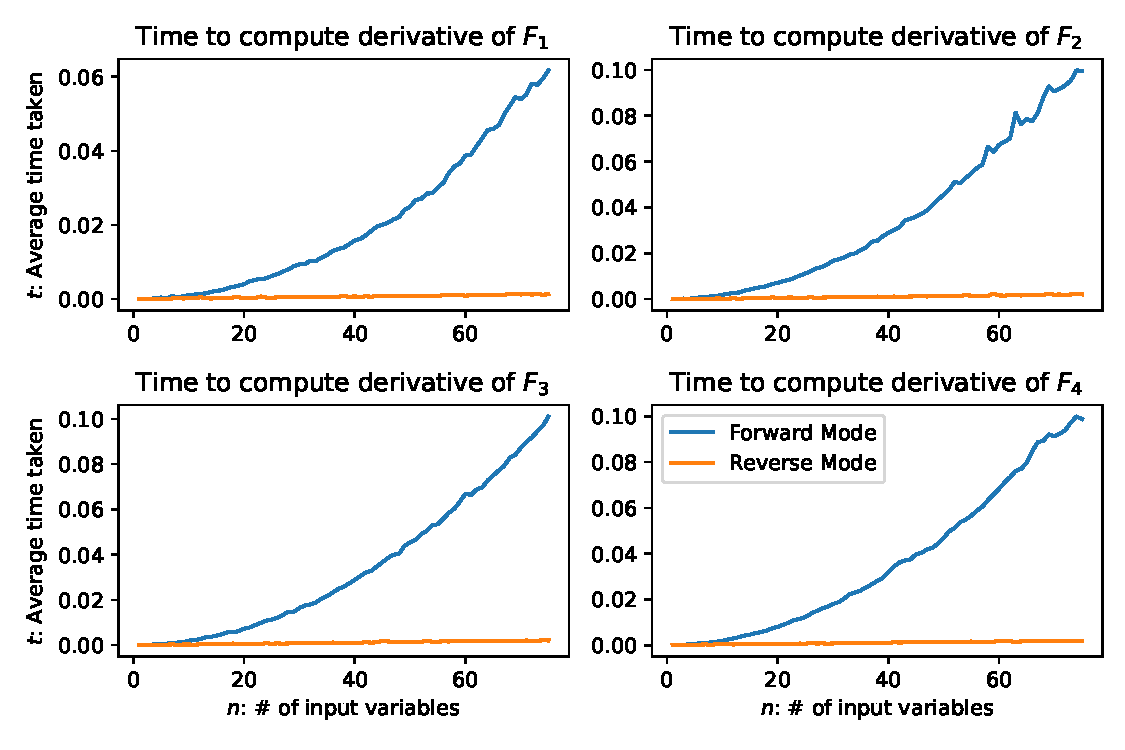
\includegraphics[width=15cm]{images/Graph_TimeDiff.pdf}
    \caption{Average time taken to compute the derivatives of the functions in \eqref{TimeFunc}, 50 times varying the number of input parameters}
    \label{fig:TimeDiff}
\end{figure}

As expected, forward mode AD grows proportionately to the number of unique input variables that we have compared to reverse mode AD which stays roughly the same, taking into account the difference in evaluating $F$ each time too. This further proves the importance of using reverse mode when working with systems where the number of input variables are several orders of magnitude greater than the number of output variables, for example, neural networks.

We can also see from \cite{github} below the heat-map of the runtime when computing the derivative of a function, $F: \mathbb{R}^n \rightarrow \mathbb{R}^m$ listed in \eqref{func_nm}.

\begin{equation}
    F \begin{pmatrix}
        x_1 \\ \vdots \\ x_n
    \end{pmatrix} = \begin{pmatrix}
        \sum_{k=1}^n 1 \cdot x_k^1 \\ \sum_{k=1}^n 2 \cdot x_{k}^{2} \\ \vdots \\ \sum_{k=1}^n m \cdot x_{k}^{m}
    \end{pmatrix}
    \label{func_nm}
\end{equation}


\begin{figure}[h]
    \centering
    \includegraphics{images/Graph_HeatmapTimeDiff.pdf}
    \caption{Heatmap of mean time taken to compute the derivative of function in \eqref{func_nm}}
    \label{fig:heatmap}
\end{figure}

Here we can see that for a function with a low number of input parameters and a high number of output variables we may prefer to use forward mode AD, however for functions with a high amount of input variables and a low number of output variables we will much prefer to use reverse mode AD. We can also see that reverse mode AD stays at low cost throughout compared to forward mode which blows up quickly with each increase in input/output variables.

\section{Implementing PDEs into Reverse Mode}

Currently we have implemented basic reverse mode algorithmic differentiation for general expressions. However what if we want to have a more complicated expression, perhaps one where one of our operators is to go and compute some PDE. This is the next extension we will be looking at. Particularly we will be looking at solving and implementing the Advection-Diffusion equation into our current system.

\subsection{Advection Diffusion Equation}

Consider the simplified 1-dimensional advection-diffusion equation \cite{AdvDiffPollutant} given by \eqref{AdvectionDiffusion} where we are measuring the concentration of some liquid over some distance over time, also accounting for the velocity of the liquid, $V$, and the rate of diffusion, $D$.

\begin{equation}
    \label{AdvectionDiffusion}
    \frac{\partial C}{\partial t} = - V\frac{\partial C}{\partial x} + D\frac{\partial^2 C}{\partial x^2}
\end{equation}

If we model concentration along the 1-dimension as a simple function of distance we can then interpolate the concentration across the domain. Below we have an example of interpolation of a function that denotes concentration distributed by the standard-normal distribution in Figure \ref{fig:sampling}.

\begin{figure}
\centering
    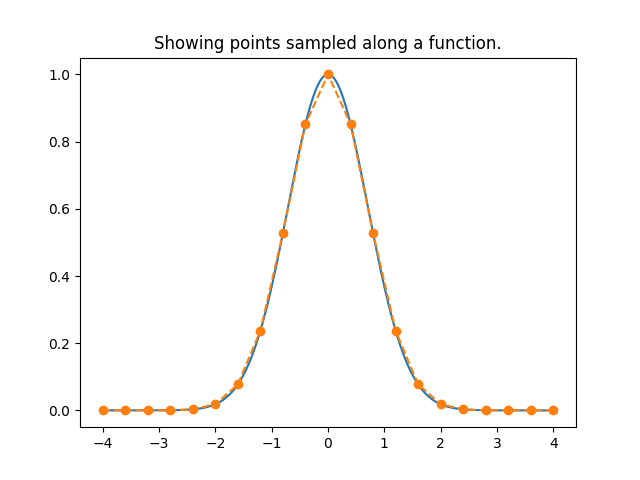
\includegraphics[width=12cm]{images/show_sampling.png}
    \caption{Difference between true function and sampled function}
    \label{fig:sampling}
\end{figure}

Now given some interpolated points, using central difference equations from \cite{numanal}, we can find approximations for $\frac{\partial C}{\partial x}$ and $\frac{\partial^2 C}{\partial x^2}$. If we number the nodes $C_1, \ldots , C_n$ for our interpolated points, using subscript to denote indexing over our spatial domain, $x$, then we get

\begin{equation} \label{pde1}
    \frac{\partial C_i}{\partial x} \approx \frac{C_{i+1} - C_{i-1}}{2h}
\end{equation}
\begin{equation} \label{pde2}
    \frac{\partial^2 C_i}{\partial x^2} \approx \frac{C_{i+1} -2C_i + C_{i-1}}{h^2}
\end{equation}

Where $h$ is the distance between each sample point. Using methods from \cite{differential}, systems \eqref{pde1} and \eqref{pde2} can be generalised for all points in \eqref{CentralDifference1} and \eqref{CentralDifference2}, respectively.
\begin{equation} \label{CentralDifference1}
        \underbrace{\frac{1}{2h}
        \begin{bmatrix}
        0 & 0 &  & & \\
        -1 & 0 & 1 & &\text{\huge{$0$}} & \\
         & -1 & 0 & \ddots &\\
         & & \ddots & \ddots & 1 \\
         & \text{\huge{$0$}} & & -1 & 0 & 1 \\
         & & & & 0 & 0
        \end{bmatrix}}_\text{\large{$A$}}
        \underbrace{\begin{bmatrix}
            C_1 \\ \vdots \\ C_n
        \end{bmatrix}}_\text{\large{$C$}}
        \approx
        \begin{bmatrix}
            \frac{\partial C_1}{\partial x} \\ \vdots \\ \frac{\partial C_n}{\partial x}
        \end{bmatrix}
\end{equation}
\begin{equation} \label{CentralDifference2}
        \underbrace{\frac{1}{h^2}
        \begin{bmatrix}
        0 & 0 &  & & \\
        1 & -2 & 1 & &\text{\huge{$0$}} & \\
         & -1 & -2 & \ddots &\\
         & & \ddots & \ddots & 1 \\
         & \text{\huge{$0$}} & & -1 & -2 & 1 \\
         & & & & 0 & 0
        \end{bmatrix}}_\text{\large{$B$}}
        \underbrace{\begin{bmatrix}
            C_1 \\ \vdots \\ C_n
        \end{bmatrix}}_\text{\large{$C$}} \approx
        \begin{bmatrix}
            \frac{\partial^2 C_1}{\partial x^2} \\ \vdots \\ \frac{\partial^2 C_n}{\partial x^2}
        \end{bmatrix}
\end{equation}

The first and last rows in both matrices are zero rows as the derivative is 0 at the boundary conditions. We denote the matrix for the first derivative as $A$ and the matrix for the second derivative as $B$. Note we also have vector $C = [C_1 \cdots C_n]^T$ which is our vector of concentration indexed at our spatial points. Now by stepping forward in time, we get the equation, we will use superscript to define indexing over time.
\begin{equation}
    C^{t+\Delta t} = C^{t} + \Delta t \frac{\partial C^{t+\Delta t}}{\partial t}
    \label{newC}
\end{equation}
We can approximate $\frac{\partial C}{\partial t}$ in \eqref{AdvectionDiffusion} using $A$ and $B$ then substituting into \eqref{newC} yields \eqref{sub}

\begin{equation} \label{sub}
    \begin{split}
        & \frac{\partial C}{\partial t} \approx -VA + DB \\
        \Longrightarrow \ & C^{t+\Delta t} = C^{t} + \Delta t (-VA + DB) C^{t+\Delta t} \\
        \Longrightarrow \ & [I + \Delta t(VA - DB)]C^{t+\Delta t} = C^{t}
    \end{split}
\end{equation}
\begin{equation} \label{CnewMCold}
    \begin{split}
        & M := I + \Delta t(VA - DB) \\
        \Longrightarrow \ &  C^{t+\Delta t} = M^{-1} C^{t}
    \end{split}
\end{equation}
Solving \eqref{CnewMCold} gives us a way of modeling the concentration in 1-dimension over time. This can be easily implemented in Python, making use of the \verb|numpy.linalg| module, particularly the \verb|solve| method.

\begin{figure}[h]
    \centering
    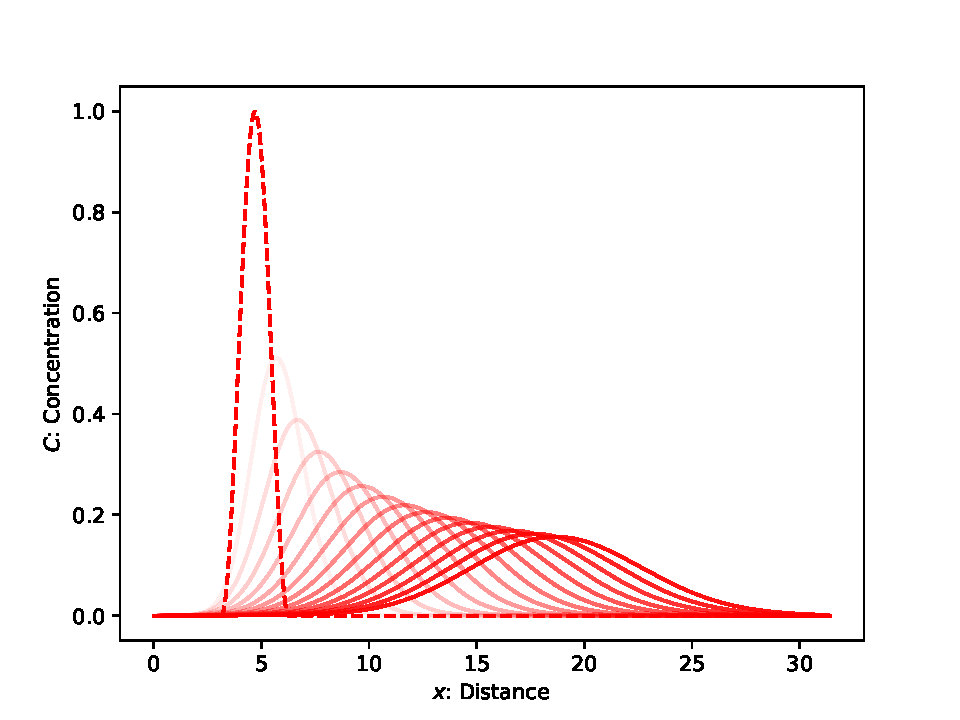
\includegraphics{images/Graph_PDE.pdf}
    \caption{Plot of \eqref{AdvectionDiffusion} with V=10, D=5, plotting each timestep of $\Delta t=0.1$ from t=0 to t=1.5, represented by lines of difference opacity. Dashed line is initial value at t=0}
    \label{fig:ODE}
\end{figure}

\subsection{Implementation}
We will apply our code to find the adjoint value $\Bar{C}^t$ from some output $\Bar{C}^{t+\Delta t}$. Calculating this value is of great importance, as it can tell us how our initial conditions will affect our final result forward in time. For example, if we were modeling how pollution spread in the sea, and the adjoint, $\Bar{C_i}^t+\mu*\Delta t$ of some point in time would tell us how much our initial pollutant map $C^t$ affected that point. This could help us know the extent to which increasing or decreasing pollution in the area will affect the surrounding environment.

To implement PDEs into our reverse mode implementation we first have to know what the adjoint of this PDE might be. We know in general if we have a function $\varphi_i$ to be defined as a matrix operator, $A$. Then the corresponding adjoint of $A$ will be its conjugate transpose \cite{adjointref}, or in the case of $A \in \mathbb{R}^n$ the adjoint is just its conjugate $A^\text{T}$ So in our case the adjoint of $M^{-1}$ will be $M^{-\text{T}}$. Here the superscript $-\text{T}$ means the inverse transpose of our matrix, as the two properties are immutable.

\begin{equation} \label{PDEadjoint}
    \begin{split}
        & M := I + \Delta t(VA - DB) \\
        \Longrightarrow \ &  \Bar{C}^{t} = M^{-\text{T}} \Bar{C}^{t+\Delta t}
    \end{split}
\end{equation}

Hence all we need to do is now implement this into our code. We first created the solve method for \eqref{AdvectionDiffusion} which would give the next solution as in \eqref{CnewMCold} of the PDE in one timestep, $\Delta t$, this is used in our evaluate method \cite{github}:

\begin{verbatim}
    def solve(C, gridpoins, dt, V, D)
        m = matrix(gridpoints, dt, V, D)
        C = np.linalg.solve(m, C)
        return C
\end{verbatim}

Where \verb|matrix()| would return the matrix we specified above in \eqref{CnewMCold}

Our \verb|evaluate()| and \verb|adjoint_evaluate()| methods are now extended \cite{github} to include this:


Here is the code we used to plot our Taylor error:

\begin{verbatim}
    @evaluate.register(expressions.AdvDif)
    def _(expr, *o, **kwargs):
        V = expr.V
        D = expr.D
        dt = expr.dt
        size = expr.size
        numpoints = len(o[0])
        gridpoints = np.linspace(0, size, numpoints)
        return solve(o[0], gridpoints, dt, V, D)
\end{verbatim}

\begin{verbatim}
    @adjoint_evaluate.register(expressions.AdvDif)
    def _(expr, *o, **kwargs):
        V = expr.V
        D = expr.D
        dt = expr.dt
        size = expr.size
        numpoints = len(o[0])
        gridpoints = np.linspace(0, size, numpoints)
        M = matrixM(gridpoints, dt, V, D)
        return [np.linalg.solve(M.T, expr.adjoint)]
\end{verbatim}

We also create a Pick function \cite{github} in our implementation which will index our output array, this allows us to see just one $C_i$ from our array, we also add this to our \verb|evaluate()| and \verb|adjoint\_evaluate()| methods. For evaluate this will simply return the $i$th element in our array, and adjoint evaluate will simply return a identity array with 0's in all places but $1*expr.adjoint$ at index $i$. Here we can choose $i$ to be any index we like.

Here we can also plot our adjoint of our PDE over each time step to see how the much the effected points change over time. The results of this plot \cite{github} are seen in Figure \ref{fig:adjointplot}

Here we see our adjoint dispersing against the direction of velocity, we see this because as the concentration is moving forward in time, and therefore move further to the right, the points which have affected this value $C_{300}$ will now be further to the left, we also see it spread out, which indicates that as the concentration spreads out, so do the points which affect it forward in time.

\begin{figure}[h!]
    \centering
    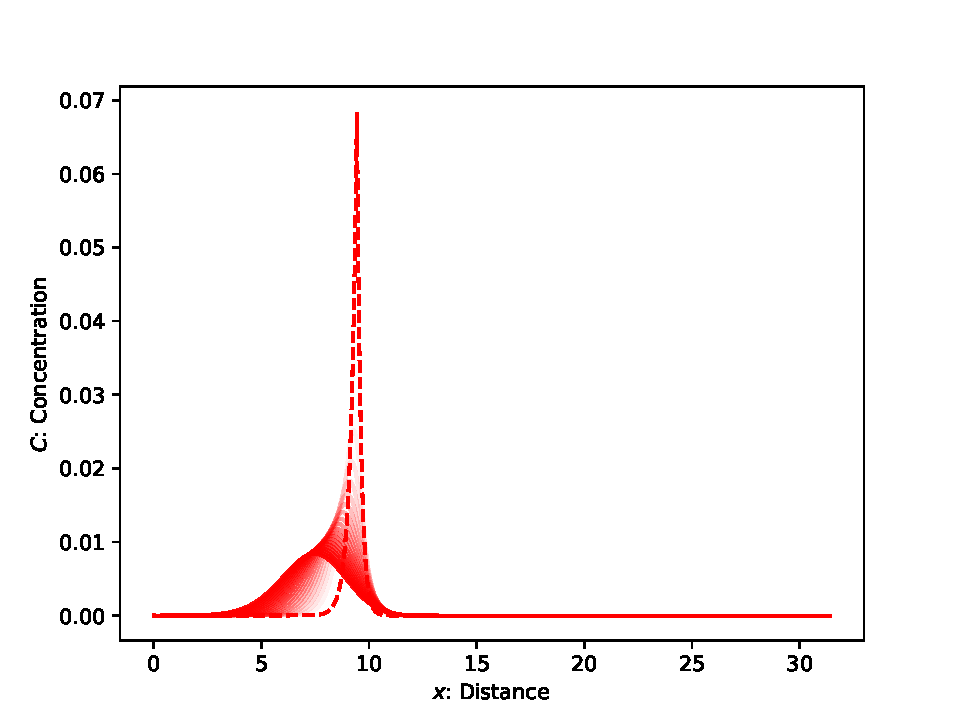
\includegraphics[width=12cm]{images/Graph_PDE_adjoint_plot.pdf}
    \caption{Plotting of the adjoint of our PDE \ref{fig:ODE} at point, $i=300$ from $t=0$ to $t=2$, plotting each timestep of $\Delta t=0.1$ from t=0 to t=1.5, represented by lines of difference opacity. Dashed line is initial value at t=0}
    \label{fig:adjointplot}
\end{figure}


\subsection{Multivariate Taylor error}

In section 8 we discussed how to find errors when we were given 1 adjoint value per variable. When working with our PDEs however we are given an array with dimension equal to the number of sampling points. In this case, we will use the equation for a multivariate Taylor Test:

\begin{equation}
    F(x + \varepsilon \cdot V) - F(x) - \varepsilon \frac{\delta F}{\delta x} \cdot V = \mathcal{O}(\varepsilon^2)
    \label{multidimtaylor}
\end{equation}

In this case, $V \in \mathbb{R}^n$ is the direction in which we take our derivative. So if we randomise $V$ then we can be certain our test is accurate. Here our function has to output a scalar value, otherwise, there will be a dimension mismatch. For this, we use the Pick function as defined in the section above.

When applying this to our Adjoint PDE, we use a single time step followed by a pick function to define our function $F: \mathbb{R}^n \rightarrow \mathbb{R}$.

To plot the Taylor error we use the following code, running this code \cite{github} gives us the plot in figure \ref{fig:ODE}.



\begin{verbatim}
    numpoints = 1000
    size = 10*np.pi
    func = lambda x: np.sin(x)**2 if np.pi <= x <= 2*np.pi else 0.0
    C0 = initial_C(func, size, numpoints)
    pick = expressions.Pick(None, e=130)
    pde = expressions.AdvDif(C0, D=5, V=10, dt=0.01, size=size)
    v = expressions.Symbol('v')
    expr = pick(pde(v))
    conditions = {v: C0}
    eps = [10**(-(i+1)) for i in range(10)]
    return taylor_error_plot(expr, conditions, eps, var=v)
\end{verbatim}

\begin{figure}[h!]
    \centering
    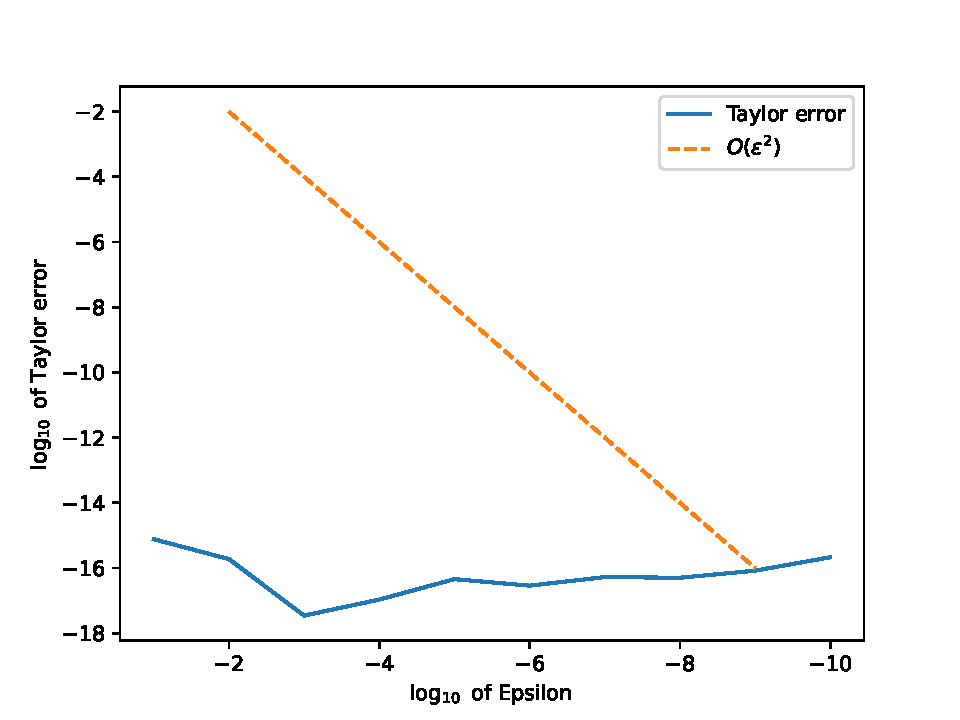
\includegraphics[width=12cm]{images/Graph_PDE_Taylor.pdf}
    \caption{Plot of Taylor error \ref{multidimtaylor} our PDE against epsilon.}
    \label{fig:ODE}
\end{figure}



Here one would initially think our result is incorrect because we don't have a convergence of order $\mathcal{O}(\varepsilon^2)$, however here we are working with a linear function so our estimation of $F(x + \varepsilon \cdot V) - F(x)$ will give an exact value for the derivative. This means when we subtract our calculation for the derivative, we should expect to get 0, which we do, the values we see in figure \ref{fig:ODE} come from a machine epsilon error.

\newpage

\section{Further Extensions}

For now, we have only included the implementation of linear PDEs \cite{github}, however, to further extend our work we could further look at implementing or trying to solve non-linear PDEs, as this would cause our adjoint to be dependent on our operand's \verb|storedvalues|, of which currently it is not. This would give a more interesting plot. Another extension to consider is checkpointing from \cite{checkpoint}, where because storing all our \verb|storedvalues| on our forward pass takes up a lot of memory, we only consider storing parts of our evaluations at set checkpoints. Hence, instead when we run our reverse pass we have to recalculate our \verb|storedvalues| from checkpoints we have stored on our forward pass. This is beneficial when calculating our \verb|storedvalues| takes considerably less time than calculating the adjoint. Also, another extension for saving memory would be to store the some, or all, of the \verb|storedvalues| into disk instead of memory. This has the drawback that storing to disk takes time, however, the amount of storage on disk is several orders of magnitude greater than memory, and in some cases theoretically infinite.

\bibliography{thebibliography}

\end{document}